\documentclass[11pt,a4paper]{article}

\usepackage[utf8]{inputenc}
\usepackage[T1]{fontenc}
\usepackage[english]{babel}
\usepackage{lmodern}
\usepackage{microtype}
\usepackage[margin=2.4cm]{geometry}
\usepackage{booktabs}
\usepackage{tabularx}
\usepackage{array}
\usepackage{xcolor}
\usepackage{enumitem}
\usepackage{float}
\usepackage{graphicx}
\usepackage{amsmath}
\usepackage{pifont}
\usepackage[round,authoryear]{natbib}
\usepackage[colorlinks=true,linkcolor=teal!70!black,citecolor=teal!70!black,urlcolor=teal!70!black]{hyperref}

\newcolumntype{Y}{>{\raggedright\arraybackslash}X}
\newcolumntype{C}[1]{>{\centering\arraybackslash}p{#1}}
\newcommand{\oui}{\textcolor{teal!70!black}{\ding{51}}}
\newcommand{\non}{\textcolor{red!60!black}{\ding{55}}}
\newcommand{\partiel}{\textcolor{orange!80!black}{$\sim$}}
\setlist{itemsep=2pt,topsep=4pt}

\title{\textbf{Route by the Evidence, Abstain in Time:\\ Adaptive Allocation of Compute and Retrieval
for Local LLMs}\\[6pt]
\large A Pre-Registered Evaluation of Quality, Latency and Energy on a Personal Computer}
\author{Alae Lahbichi\\[2pt]
\small Fifth-year student, Artificial Intelligence and Data Science\\
\small\href{mailto:a.lahbichi2004@gmail.com}{\texttt{a.lahbichi2004@gmail.com}}\\
\small Code and data: \href{https://github.com/AlaeLahbichi/Adaptive-Compute-and-RAG-for-Efficient-Reliable-Local-LLMs}{\scriptsize\texttt{github.com/AlaeLahbichi/Adaptive-Compute-and-RAG-for-Efficient-Reliable-Local-LLMs}}}
\date{October 2026}

\begin{document}
\maketitle

\begin{abstract}
\noindent Running a language model on one's own machine keeps one's data at home, but every answer is
paid for in seconds of waiting and in joules. Yet not every question deserves the same effort: some
can be settled without any document, others call for a larger model and several passages, and others
still have no answer in the corpus, in which case the only honest reply is to abstain. This paper
studies how to make these three decisions jointly, question by question, from signals that cost almost
nothing. We propose a policy that relies on evidence sufficiency, measured by the BM25 score of the
best passage, and on model confidence, read from the probabilities of the tokens it produces. We
evaluate it on an Apple M3 Pro with two 4-bit quantised Qwen models, on a 630-question benchmark built
from SQuAD 2.0 and HotpotQA, fixing our success criteria before any experiment and running the test set
only once. On 450 test questions, the policy matches the quality of the reference configuration (score
0.550 versus 0.537, non-inferiority demonstrated), makes fewer errors and outperforms two routers
inspired by prior work. It reduces latency by only 10\% and energy by 9\%, however, where we aimed for
20\%: the primary criterion is not met. We show that this gap stems from tuning an absolute threshold
on too small a sample, and we derive a precise programme of improvements.

\medskip
\noindent\textbf{Keywords:} local language models, model routing, adaptive RAG, abstention, energy
efficiency, pre-registered evaluation.
\end{abstract}

%======================================================================
\section{Introduction}\label{sec:intro}
%======================================================================

\subsection{Context}

Until recently, querying a large language model meant sending one's question to a remote server. That
is no longer the case. Models with a few billion parameters, once quantised, fit in the memory of a
laptop and answer in under a second. This shift changes the nature of the problem. A company that wants
to query its archives without handing them to a third party, a researcher working with sensitive data,
a student with no budget for an API: all of them can now have a local assistant. In return, the cost of
each answer stops being an abstract line on an invoice. It becomes waiting time, occupied memory and
drained battery.

Two levers improve the answers of such a system, and both come at a price. The first is model size: a
larger model reasons better, but it is slower. The second is document retrieval, or retrieval-augmented
generation (RAG): by attaching passages from a corpus to the question, the answer is grounded in sources
and the model invents less \citep{gao2023ragsurvey}. But every added passage lengthens the text the
model must read, and hence the computation time. Finally, there is a third option that is often
forgotten: not answering. When the documents do not contain the requested information, a frank
abstention is better than a plausible but wrong answer \citep{wen2024abstention}.

\subsection{Problem statement}

Common practice is to fix a configuration once and for all, for instance ``the largest available model
with three passages'', and to apply it to every question. This choice is convenient but doubly
inefficient. On a simple question whose answer appears verbatim in a passage, it mobilises an oversized
model. On a question the corpus cannot answer, it spends a full generation to produce, at best, an
admission of ignorance and, at worst, an error. Conversely, always choosing the lightest configuration
sacrifices quality on hard questions.

The problem is therefore one of \emph{allocation}: giving each question the resources it needs, no more
and no less. It is a delicate one for three reasons. First, the decision must be made \emph{before} the
answer is known, from imperfect clues. Second, these clues have a cost of their own: a decision signal
that requires an extra generation may cancel out the saving it is meant to produce. Third, the objective
is multiple. We want to reduce latency and energy, but without losing quality, without increasing
errors and without sacrificing one category of questions for another. We thus state the problem
addressed in this work:

\begin{quote}
\emph{How can computational and retrieval resources be allocated automatically and measurably to each
query, so as to reduce the cost of a local question-answering system without significantly degrading
the quality, factuality and reliability of its answers?}
\end{quote}

\subsection{Research questions}

This problem breaks down into four questions, which structure the rest of the paper.

\begin{description}[style=sameline,leftmargin=1.2cm]
\item[RQ1] Can an inexpensive signal be used to choose the model and the level of retrieval without
loss of quality?
\item[RQ2] Can the decision to abstain be made reliably by combining model uncertainty and the quality
of the retrieved evidence?
\item[RQ3] What trade-off between quality, latency and energy is actually achieved on a personal
computer, once the cost of the decision signals is counted?
\item[RQ4] Are the gains homogeneous across question types, or are some profiles sacrificed?
\end{description}

\subsection{Approach and contributions}

We addressed these questions step by step, under strict experimental discipline. A literature review
first situated the problem and led to our hypotheses. We then built a benchmark and a protocol, and
wrote down our success criteria \emph{before} any experiment. A pilot study validated the measurement
chain. Reference methods, fixed or inspired by published work, set the bar. We then designed and tuned
an adaptive policy on a development set, before freezing it and evaluating it once on a test set never
consulted before. This work makes five contributions:

\begin{enumerate}
\item a synthesis of the literature showing that model choice, the retrieval decision and abstention
are almost always treated separately, with costs rarely measured on local hardware;
\item a pre-registered benchmark and protocol, with latency measured over three passes and energy
measured with \texttt{powermetrics};
\item a set of reference methods: six fixed strategies and two routers inspired by RouteLLM and
Adaptive-RAG;
\item a joint adaptive policy, simple and interpretable, built on nearly free signals;
\item a final evaluation whose partially negative outcome we report honestly, together with an analysis
of its causes and concrete avenues for improvement.
\end{enumerate}

\paragraph{Outline.} Section~\ref{sec:cadre} defines the notions used throughout. Section~\ref{sec:etat}
reviews the state of the art and derives our hypotheses. Section~\ref{sec:protocole} describes the
benchmark and protocol, Section~\ref{sec:pilote} the pilot study, Section~\ref{sec:references} the
reference methods and Section~\ref{sec:politique} the adaptive policy. Section~\ref{sec:final} reports
the final evaluation. We discuss the results in Section~\ref{sec:discussion}, examine the weaknesses of
the study in Section~\ref{sec:faiblesses}, and conclude in Section~\ref{sec:conclusion}.

%======================================================================
\section{Conceptual framework}\label{sec:cadre}
%======================================================================

Several terms recur throughout this paper. We clarify them here, as their usage varies from one work to
another.

\textbf{Routing} means choosing, before any generation, which model will handle a query among several
candidates of different sizes or costs. A \textbf{cascade} is a sequential variant: an inexpensive model
is queried first, and a more powerful one takes over if the first answer looks unreliable. The cost of
the first model is paid in every case, which weighs heavily when escalation is frequent.

\textbf{Retrieval-augmented generation} (RAG) adds to the prompt passages extracted from a document
collection. RAG is called \textbf{adaptive} when it decides, query by query, whether to retrieve, when
to retrieve and how many passages to keep.

\textbf{Uncertainty} refers to an estimate of the probability that an answer is wrong. It can be read
from the model's internal probabilities, from the consistency between several sampled answers, or from
the confidence the model expresses itself. The \textbf{evidence} is the set of retrieved passages; its
\textbf{sufficiency} measures the extent to which they seem to contain what is needed to answer.

\textbf{Abstention} is the refusal to answer when the risk of error is judged too high. It is evaluated
through two complementary quantities \citep{kamath2020selective}: \textbf{coverage}, the share of
questions the system answers, and \textbf{risk}, the share of wrong answers among those it gives.
Abstaining more lowers coverage; it is worthwhile if risk falls accordingly.

Finally, \textbf{cost} does not mean the same thing everywhere. Depending on the work, it is the price
charged by an API, the number of calls to the large model, the number of tokens, latency, memory or
energy. These measures are not interchangeable. In this work, cost is what the user of a personal
machine experiences: end-to-end latency and the energy consumed by the chip, complemented by the number
of tokens.

%======================================================================
\section{State of the art}\label{sec:etat}
%======================================================================

\subsection{Review method}

We searched arXiv, the ACL Anthology, OpenReview, Google Scholar and Semantic Scholar, as well as the
proceedings of NeurIPS, ICLR, AAAI and MLSys. Queries combined the notions of the topic and their
synonyms: \textit{LLM routing}, \textit{model cascade}, \textit{adaptive retrieval}, \textit{adaptive
RAG}, \textit{uncertainty estimation}, \textit{selective prediction}, \textit{abstention} and
\textit{energy-aware inference}. We kept works that adapt, query by query, the choice of model,
retrieval or the decision to answer, provided they include an experimental evaluation, as well as
studies of inference cost and datasets useful for our protocol. Infrastructure work, position papers
without experiments and multi-agent systems outside question answering were excluded. Starting from
seventeen references, we identified fifty-one by following citations in both directions and running a
targeted search for 2025 and 2026 work; forty-six were retained and grouped by theme.

\subsection{Model routing and cascades}

The idea of reserving the large model for queries that warrant it is not new, but it gained momentum
with the spread of paid APIs. \citet{chen2023frugalgpt} give a general formulation with FrugalGPT,
which chains models of increasing cost and stops as soon as a learned scorer deems the answer
acceptable; they report considerable savings at equal quality. AutoMix \citep{aggarwal2023automix}
replaces this scorer with a self-verification by the small model, whose noise is absorbed by a Markov
decision process. \citet{yue2023cascades} use another clue: when several answers from the small model
agree, it is likely to be right.

A second family decides \emph{before} any generation. Hybrid LLM \citep{ding2024hybrid} predicts the
difficulty of a query to send it to the small or the large model, with a threshold adjustable at
inference time. RouteLLM \citep{ong2024routellm} learns this choice from human preferences and shows
that the resulting routers transfer to other model pairs. Other work relies on a multi-armed bandit
\citep{nguyen2024metallm} or a reward model \citep{lu2023zooter}. To compare these approaches,
RouterBench \citep{hu2024routerbench} offers a common evaluation framework.

The most recent work refines the notions of cost and guarantee. \citet{fu2026inflation} show that the
cost of a single call greatly underestimates that of a workflow that retries queries, and propose a
difficulty signal computed locally before execution. RACER \citep{hao2026racer} produces sets of models
with a calibrated threshold that allows abstention and controls the risk of routing errors, with
guarantees that make no assumption about the data distribution. The survey by \citet{varangot2025survey}
takes stock of the field and points out two weaknesses: poorly standardised experimental protocols and
an almost exclusive focus on financial cost.

\subsection{Adaptive RAG}

That retrieval is not always useful was shown convincingly by \citet{mallen2022trust}: models retain
popular knowledge well and rare knowledge poorly, so retrieving only when necessary improves both
accuracy and cost. The methods that followed differ mainly in the clue that triggers retrieval. SKR
\citep{wang2023skr} relies on what the model knows about itself; FLARE \citep{jiang2023flare} and DRAGIN
\citep{su2024dragin} trigger retrieval mid-generation, as soon as the model hesitates; Self-RAG
\citep{asai2023selfrag} teaches the model to emit reflection tokens that judge passage relevance, at the
cost of dedicated training.

Adaptive-RAG \citep{jeong2024adaptiverag} is the reference closest to our problem. A small classifier
predicts the complexity of the question and chooses between no retrieval, single-step retrieval and
iterative retrieval. HyPA-RAG \citep{kalra2024hyparag} transposes this idea to retrieval parameters in
the legal domain. Other work judges the documents rather than the question: Corrective RAG
\citep{yan2024crag} evaluates the retrieved passages and decides whether to use, supplement or discard
them, and Tiny-Critic RAG \citep{wu2026tinycritic} delegates this check to a small model to reduce its
latency.

A comparative study by \citet{moskvoretskii2025adaptive} particularly shaped our work: across some
thirty methods, simple uncertainty estimators rival far more complex pipelines and often beat them on
efficiency. More recently, Self-Routing RAG \citep{wu2025srrag} treats the model itself as one knowledge
source among others, RAGRouter-Bench \citep{wang2026ragrouterbench} frames the choice of a RAG paradigm
as a routing problem, and Pre-Route \citep{chen2026preroute} arbitrates between RAG and long context.
Finally, several works reduce the cost of the context itself by keeping only the useful sentences
\citep{arefeen2024leancontext,akesson2024clustered,chen2026logicrag}.

\subsection{Uncertainty and abstention}

To decide to abstain, one must first know when the model is likely to be wrong.
\citet{kadavath2022know} show that large models are often well calibrated when asked to judge their own
answers. Semantic entropy \citep{kuhn2023semantic} and SelfCheckGPT \citep{manakul2023selfcheckgpt}
compare several sampled answers: their disagreement betrays uncertainty or hallucination. These signals
are effective, but they require several generations per question, which makes them costly precisely in
the setting that concerns us. Confidence expressed in words by the model, for its part, is reliable only
after specific training \citep{lin2022verbal}.

\citet{kamath2020selective} laid the foundations of selective question answering, with the notions of
coverage and risk that we adopt, and showed that a learned calibrator outperforms raw probabilities,
which are overconfident outside the training domain. The survey by \citet{wen2024abstention} observes
that abstention is still rarely integrated into RAG systems as a decision in its own right.

\subsection{Cost and energy of inference}

\citet{samsi2023watts} measured the inference energy of LLaMA as a function of model size on
data-centre GPUs. \citet{luccioni2022bloom} estimated the carbon footprint of BLOOM over its whole life
cycle, and \citet{luccioni2024power} compared the energy cost of many models and tasks, showing that
general-purpose generative models are far more demanding than specialised ones. These works
\emph{measure} energy, but none seeks to \emph{reduce} it through per-query decisions, and all concern
data-centre hardware.

\subsection{Datasets and evaluation practices}

Available datasets cover the question profiles we are interested in well. SQuAD 2.0
\citep{rajpurkar2018squad2} provides single-answer questions and unanswerable questions; HotpotQA
\citep{yang2018hotpotqa} and MuSiQue \citep{trivedi2022musique} provide questions that require combining
several documents; the CRAG Benchmark \citep{yang2024cragbench} provides varied questions where
hallucinations are penalised. Methodologically, two lessons seemed essential to us. First,
\citet{li2026beyond} show that retrieval-derived signals, although correlated with the usefulness of an
extra step, do not reliably improve a router that reads only the question: any new signal must therefore
be compared against such a control. Second, RouterBench and RAGRouter-Bench evaluate quality and cost as
a trade-off rather than with a single metric, which we do as well.

\subsection{Synthesis and positioning}

Table~\ref{tab:positionnement} situates the closest works with respect to the three decisions of
interest.

\begin{table}[H]
\centering\footnotesize
\setlength{\tabcolsep}{3.5pt}
\begin{tabularx}{\textwidth}{l C{1.2cm} C{1.2cm} C{1.3cm} Y Y C{0.9cm}}
\toprule
\textbf{Work} & \textbf{Model choice} & \textbf{RAG decision} & \textbf{Abs\-ten\-tion} & \textbf{Decision signal} & \textbf{Cost evaluated} & \textbf{Local} \\
\midrule
FrugalGPT & \oui & \non & \non & Learned scorer (after generation) & API price & \non \\
Hybrid LLM & \oui & \non & \non & Predicted difficulty (before) & Large-model calls & \partiel \\
RouteLLM & \oui & \non & \non & Human preferences & Price, calls & \non \\
AutoMix & \oui & \non & \non & Self-verification (after) & Compute & \non \\
RACER & \oui & \non & \oui & Calibrated score & Set size & \non \\
Adaptive-RAG & \non & \oui & \non & Question complexity & Time, steps & \non \\
Corrective RAG & \non & \oui & \non & Document quality & -- & \non \\
Moskvoretskii et al. & \non & \oui & \non & Uncertainty & Calls, retrievals & \non \\
RAGRouter-Bench & \partiel & \oui & \non & Query--corpus fit & Resources & \non \\
Kamath et al. & \non & \non & \oui & Learned calibrator & -- & \non \\
\midrule
\textbf{This work} & \oui & \oui & \oui & \textbf{BM25 evidence and confidence, cost counted} & \textbf{Latency, tokens, energy} & \oui \\
\bottomrule
\end{tabularx}
\caption{Positioning of the closest works. \oui{}: addressed; \non{}: not addressed; \partiel{}:
partially.}
\label{tab:positionnement}
\end{table}

Four gaps emerge from this review. The three decisions are almost always made \emph{in isolation}: the
model is chosen without regard to retrieval, or vice versa, and abstention is studied separately. Cost
is mostly \emph{financial}, rarely measured on the user's machine. The cost of the signals themselves,
whether several generations or a judge model, is rarely subtracted from the reported gain. Finally,
evaluation is sometimes optimistic: a ``question-only'' control is often missing, and a global average
can hide losses on one category of questions. Table~\ref{tab:distinction} specifies what distinguishes
our work from the closest ones.

\begin{table}[H]
\centering\small
\begin{tabularx}{\textwidth}{l Y Y}
\toprule
\textbf{Work} & \textbf{What it already does} & \textbf{What remains open} \\
\midrule
Adaptive-RAG & Question complexity $\rightarrow$ retrieval strategy & Model choice, abstention, local measurement \\
Moskvoretskii et al. & Simple uncertainty signals to decide on retrieval & Several model sizes, abstention, energy \\
RAGRouter-Bench & Routing between RAG paradigms with resource cost & Abstention, local hardware, joint decision \\
Fu et al. (2026) & Local pre-execution signal, real cost & Adaptive retrieval, abstention \\
RACER & Routing with calibrated abstention & Retrieval, local cost \\
\bottomrule
\end{tabularx}
\caption{What distinguishes this work from the closest ones.}
\label{tab:distinction}
\end{table}

These observations led us to four working hypotheses, which answer the research questions of the
introduction.

\begin{description}[style=sameline,leftmargin=1cm]
\item[H1] An inexpensive signal computed before generation can direct a significant share of queries to
the small model without loss of quality beyond the set margin.
\item[H2] Combining model uncertainty and evidence sufficiency improves the coverage--risk trade-off
compared with either signal alone.
\item[H3] A joint policy dominates fixed strategies on the quality--cost curve, including the cost of
its own signals.
\item[H4] Gains vary by question category and must therefore be reported per category.
\end{description}

%======================================================================
\section{Benchmark and protocol}\label{sec:protocole}
%======================================================================

\subsection{Building the benchmark}

We built a benchmark from two public datasets, both licensed under CC BY-SA 4.0, whose SHA-256
fingerprints are checked at every build. The SQuAD 2.0 development set \citep{rajpurkar2018squad2}
covers thirty-five Wikipedia articles and mixes answerable questions with unanswerable ones written to
resemble them. The HotpotQA development set in the \emph{distractor} setting \citep{yang2018hotpotqa}
contains questions that require combining two Wikipedia pages.

The document corpus is the library that retrieval draws from; it is not used to train the models. It
gathers the 1,204 paragraphs of SQuAD 2.0 and the 2,089 paragraphs associated with the selected HotpotQA
questions, i.e.\ 3,293 passages. All questions query this same corpus, so retrieval must find the right
passages among several thousand.

Questions fall into three balanced categories (Table~\ref{tab:benchmark}). \emph{Simple} questions find
their answer in a single passage; \emph{complex} questions require combining two; \emph{uncovered}
questions have no answer in their source paragraph, and the expected behaviour is then to abstain. To
avoid any leakage between tuning and evaluation, SQuAD questions are split \emph{by article}: no
paragraph is ever used for both development and test. We had planned a fourth category of ambiguous
questions, to be written by hand; it could not be built in time.

\begin{table}[H]
\centering\small
\begin{tabularx}{\textwidth}{l l Y l c c}
\toprule
\textbf{Category} & \textbf{Source} & \textbf{Definition} & \textbf{Expected} & \textbf{Dev} & \textbf{Test} \\
\midrule
Simple & SQuAD 2.0 & The answer lies in a single passage & Answer & 60 & 150 \\
Complex & HotpotQA & The answer requires combining two passages & Answer & 60 & 150 \\
Uncovered & SQuAD 2.0 & The source passage does not contain the answer & Abstain & 60 & 150 \\
\midrule
\multicolumn{4}{l}{\textbf{Total}} & 180 & 450 \\
\bottomrule
\end{tabularx}
\caption{Benchmark categories and split between development and test (seed 2026).}
\label{tab:benchmark}
\end{table}

\subsection{Environment and generation}

All experiments were run on an Apple M3 Pro with 12 cores and 18~GB of unified memory, using Python 3.12
and the MLX library. We use two 4-bit quantised models preloaded in memory: Qwen2.5-1.5B-Instruct, which
we call the \emph{small} model, and Qwen3-4B-Instruct-2507, the \emph{large} one. Exact model revisions
are recorded in the repository. Decoding is greedy and limited to 32 tokens, so outputs are fully
deterministic. Prompts are identical for all systems and contain an explicit abstention instruction:
reply exactly \texttt{UNANSWERABLE} when the answer is unknown or absent from the passages. Three
warm-up requests precede each series.

\subsection{Measurements}

The main metric is a \emph{global score} computed for each question. When an answer is expected, it is
the lexical F1 between the produced answer and the best reference answer. For an uncovered question, it
is 1 if the system abstains and 0 otherwise. An answer is considered correct when its F1 reaches 0.5,
which allows coverage and risk to be computed. Latency is measured end to end, including retrieval and
signals, with a monotonic clock; we report its mean and 95th percentile. Energy is measured with
\texttt{powermetrics}, which samples the power of the CPU, GPU and neural engine every 200~ms; it is
integrated over the duration of each series.

95\% confidence intervals are obtained by bootstrap over 10,000 resamplings of the questions. Since all
systems answer the same questions, differences between systems are computed question by question and
resampled together. Per-category results are systematically reported alongside the average.

\subsection{Pre-registered success criteria}

We wrote and published the following criteria before any experiment, to prevent ourselves from
redefining success after the fact.

\begin{center}
\fcolorbox{teal!60!black}{teal!5}{\parbox{0.92\textwidth}{
\textbf{Primary criterion.} On the test set and relative to reference strategy B (large model with
three passages), mean latency must drop by at least 20\% and the global score must not lose more than
2~points. Non-inferiority is claimed only if the upper bound of the 95\% confidence interval of the loss
stays below 2~points.\\[3pt]
\textbf{Secondary criteria.} Risk must be lower than that of B; the method must outperform a router that
reads only the question; no category may lose more than 5~points.\\[3pt]
\textbf{Negative result.} If the primary criterion is not met, the result is reported as is, with an
analysis of its causes.}}
\end{center}

All tuning is done on the development set. The protocol was frozen in a versioned configuration (Git
tag \texttt{protocole-v1.0}), followed by the adaptive policy (tag \texttt{politique-v1.0}), before the
test set was read. The test set was run only once.

%======================================================================
\section{Pilot study}\label{sec:pilote}
%======================================================================

Before investing in an adaptive method, we wanted to check that the problem was worth it. A pilot study
therefore ran four fixed strategies on the development set, with dense retrieval based on multilingual
MiniLM embeddings.

\begin{table}[H]
\centering\small
\begin{tabular}{l c c c c c c}
\toprule
\textbf{Strategy} & \textbf{Score} & \textbf{Cov.} & \textbf{Risk} & \textbf{Latency} & \textbf{Tokens} & \textbf{Energy / q.} \\
\midrule
A -- large model, no RAG & 0.313 & 0.31 & 0.82 & 0.25 s & 62 & 3.8 J \\
B -- large model with RAG  & \textbf{0.424} & 0.56 & 0.53 & 0.99 s & 579 & 22.8 J \\
C -- small model, no RAG & 0.233 & 0.46 & 0.93 & 0.13 s & 84 & 1.9 J \\
D -- small model with RAG  & 0.298 & 0.78 & 0.71 & 0.39 s & 601 & 8.6 J \\
\midrule
\textit{Oracle} & \textit{0.623} & -- & -- & \textit{0.30 s} & -- & -- \\
\bottomrule
\end{tabular}
\caption{Pilot study on the development set (180 questions, dense retrieval). The oracle picks, for
each question, the cheapest strategy that achieves the best score.}
\label{tab:pilote}
\end{table}

The pilot first confirmed that the stakes are real. Strategy B is nearly eight times slower than
strategy C and uses twelve times more energy; RAG increases both computation time and drawn power, which
rises from about 17 to 24~W. It then showed that no fixed strategy dominates everywhere: B wins on simple
questions, D on complex ones and A on uncovered ones. The oracle, which would pick the right strategy for
each question, would reach 0.62 in 0.30~s. This bound is unreachable in practice, but it measures the
available margin.

Two observations guided what followed. Abstention left to the prompt alone is poorly calibrated: the
small model with RAG almost always answers, with a risk of 0.71, while the large model without RAG
abstains on 69\% of questions. The decision to abstain must therefore belong to the policy rather than
to the model alone. Moreover, dense retrieval is the weak link for complex questions: both useful
passages are retrieved together in only 22\% of cases.

%======================================================================
\section{Reference methods}\label{sec:references}
%======================================================================

\subsection{Choice of retrieval}

The pilot prompted us to reconsider retrieval. On the development set, we compared dense retrieval,
lexical BM25 retrieval ($k_1 = 1.5$, $b = 0.75$) and a hybrid retrieval that fuses both rankings by
reciprocal rank fusion.

\begin{table}[H]
\centering\small
\begin{tabular}{l c c c c c c c}
\toprule
& \multicolumn{3}{c}{\textbf{Simple}} & \multicolumn{3}{c}{\textbf{Complex}} & \\
\cmidrule(lr){2-4}\cmidrule(lr){5-7}
\textbf{Method} & @1 & @3 & @6 & @1 & @3 & @6 & \textbf{Time / query} \\
\midrule
Dense   & 0.48 & 0.60 & 0.70 & 0.00 & 0.22 & 0.35 & 7.4 ms \\
\textbf{BM25} & \textbf{0.65} & \textbf{0.82} & \textbf{0.87} & 0.00 & \textbf{0.37} & \textbf{0.50} & \textbf{0.2 ms} \\
Hybrid & 0.60 & 0.72 & 0.80 & 0.00 & 0.33 & 0.48 & 7.1 ms \\
\bottomrule
\end{tabular}
\caption{Retrieval recall on the development set. For a complex question, both useful passages must be
retrieved, so recall@1 is zero by construction.}
\label{tab:recherche}
\end{table}

BM25 clearly wins on answerable questions, at every depth, while being forty times faster. Hybrid
retrieval finds the source paragraph of uncovered questions slightly more often, but this matters little
for them, since the expected behaviour is to abstain. The result is explained by the nature of the
questions, rich in proper nouns taken from the source text, and by the modest embedding model. We
therefore adopted BM25 and froze this choice in the protocol.

\subsection{Six fixed strategies}

We complemented the four pilot strategies with two six-passage strategies, so as to have a sufficiently
rich decision space.

\begin{table}[H]
\centering\footnotesize\setlength{\tabcolsep}{4pt}
\begin{tabular}{l c c c c c c c c}
\toprule
\textbf{Strategy} & \textbf{Score} & \textbf{95\% CI} & \textbf{Simple} & \textbf{Complex} & \textbf{Uncov.} & \textbf{Cov.} & \textbf{Risk} & \textbf{Latency} \\
\midrule
A -- large, 0 passages   & 0.312 & [0.248, 0.378] & 0.07 & 0.09 & 0.78 & 0.31 & 0.82 & 0.25 s \\
B -- large, 3 passages  & \textbf{0.541} & [0.472, 0.610] & 0.68 & 0.36 & 0.58 & 0.62 & 0.39 & 0.92 s \\
C -- small, 0 passages   & 0.233 & [0.174, 0.294] & 0.05 & 0.07 & 0.58 & 0.46 & 0.93 & 0.13 s \\
D -- small, 3 passages  & 0.330 & [0.267, 0.397] & 0.48 & 0.29 & 0.22 & 0.83 & 0.69 & 0.37 s \\
E -- large, 6 passages  & 0.570 & [0.501, 0.637] & 0.70 & 0.45 & 0.57 & 0.67 & 0.40 & 1.63 s \\
F -- small, 6 passages  & 0.372 & [0.308, 0.439] & 0.53 & 0.37 & 0.22 & 0.89 & 0.66 & 0.62 s \\
\bottomrule
\end{tabular}
\caption{Fixed strategies with BM25 on the development set (180 questions). The Simple, Complex and
Uncov.\ columns give the per-category score.}
\label{tab:strategies}
\end{table}

With BM25, reference B rises from 0.424 to 0.541: the bar the adaptive method must clear has thus been
raised. Strategy E improves on B by 2.9 points, mostly on complex questions, but at the price of 76\%
more latency, and the difference is not significant. Wider retrieval helps only part of the questions,
which argues for a case-by-case decision.

\subsection{Reference routers}

For any success of our method to be meaningful, it had to be confronted with routers drawn from the
literature. We built two, which read only the question text, represented by word and word-pair TF-IDF
features complemented with a few simple indicators (length, proper nouns, digits, question word). Since
generation is deterministic, a router's answer is that of the strategy it chooses; its computation time
is added to the latency.

The first, \textbf{R1}, follows the spirit of RouteLLM and Hybrid LLM and serves as the
``question-only'' control in the sense of \citet{li2026beyond}. A ridge regression predicts, for each
strategy $s$, the score $\hat{y}_s(q)$ it would obtain on question $q$, and the router picks
$\arg\max_s \hat{y}_s(q) - \lambda\,\bar{t}_s$, where $\bar{t}_s$ is the mean latency of $s$. We keep
the best setting that is at least 20\% faster than B ($\lambda = 0.113$). The second, \textbf{R2}, is a
simplified version of Adaptive-RAG \citep{jeong2024adaptiverag}: a logistic regression predicts the
question's complexity and chooses, with the large model, between no retrieval, three passages and six
passages.

\begin{table}[H]
\centering\small
\begin{tabular}{l c c c c c c}
\toprule
\textbf{Method} & \textbf{Score} & \textbf{Gap to B} & \textbf{95\% CI of gap} & \textbf{Latency} & \textbf{Cov.} & \textbf{Risk} \\
\midrule
B -- reference & 0.541 & -- & -- & 0.92 s & 0.62 & 0.39 \\
R1 -- question only & 0.425 & $-11.6$ & $[-18.5, -4.8]$ & 0.74 s & 0.58 & 0.57 \\
R2 -- simplified Adaptive-RAG & 0.522 & $-1.9$ & $[-7.4, +3.3]$ & 0.85 s & 0.49 & 0.39 \\
\textit{Oracle (A to F)} & \textit{0.762} & $+22.1$ & $[+16.5, +27.8]$ & \textit{0.40 s} & 0.58 & 0.19 \\
\bottomrule
\end{tabular}
\caption{Reference routers, five-fold cross-validation on the development set.}
\label{tab:routeurs}
\end{table}

The verdict on R1 is unequivocal: when forced to be 20\% faster than B, it loses almost twelve points.
On this benchmark, the wording of the question does not predict which strategy will succeed. R2 keeps
the quality of B but saves only 8\% of latency, and never chooses the small model. Meanwhile, the oracle
shows that one could gain twenty-two points while more than halving latency. The conclusion is clear: an
adaptive method must look beyond the question, starting with what retrieval has found.

%======================================================================
\section{An evidence-based adaptive policy}\label{sec:politique}
%======================================================================

\subsection{Two nearly free signals}

The first signal measures \emph{evidence sufficiency}. For a question $q$, BM25 retrieval returns the
score $S_1$ of the best passage. This raw score depends on the length and rarity of the question's
words; we therefore normalise it by the maximum score a passage could reach:
\[
\text{evidence}(q) \;=\; \frac{S_1}{\sum_{t \in q} \mathrm{idf}(t)\,(k_1+1)} \;\in\; [0,1].
\]
A value close to 1 indicates that a passage contains all the important words of the question. This
signal is a by-product of retrieval and costs only 0.2~ms.

The second signal is \emph{model confidence}. During decoding, we record the probability of each
generated token and keep either their geometric mean or their minimum. Decoding is not altered: we
checked that answers remain identical to those of the fixed strategies. Table~\ref{tab:auc} shows how
well these signals separate right answers from wrong ones.

\begin{table}[H]
\centering\small
\begin{tabular}{l l c}
\toprule
\textbf{Signal} & \textbf{Prediction target} & \textbf{AUC} \\
\midrule
Small-model confidence, 3 passages & Its answer is correct & 0.74 \\
Large-model confidence, 3 passages & Its answer is correct & 0.63 \\
Large-model confidence, 6 passages & Its answer is correct & 0.70 \\
BM25 evidence & B's answer is correct & 0.55 \\
Low BM25 evidence & The question is uncovered & 0.62 \\
\bottomrule
\end{tabular}
\caption{Predictive power of the signals on the development set (AUC of 0.5 for chance, 1 for perfect
prediction).}
\label{tab:auc}
\end{table}

These signals are informative, but no more: none exceeds 0.74. They must therefore be combined with care.

\subsection{The policy}

The policy handles each question in a few steps. It first runs a six-passage BM25 retrieval and computes
the evidence. If the evidence is below a threshold $\tau_0$, it abstains immediately, without any
generation: this is \emph{early abstention}. Otherwise, it may optionally query the small model with
three passages and keep its answer if its confidence exceeds a threshold $\tau_p$; this is the
\emph{cascade}. Failing that, it queries the large model, with six passages if the evidence is below
$\tau_k$ and three otherwise. Finally, it abstains if the large model admits ignorance or if its
confidence falls below $\tau_a$: this is \emph{final abstention}. The cost of every step actually
executed, signals included, is counted in the latency.

\subsection{Tuning and design}

Because outputs are deterministic, the policy's answer to a question is that of the step where it stops.
Computing the outputs of each step once is therefore enough to simulate the policy exactly, latencies
included, under any setting. We thus explored 246,510 settings (confidence type, thresholds, cascade or
not) and kept the one that maximises the global score subject to a mean latency of at most 78\% of B's.
The two-point margin relative to the 80\% criterion was meant to protect against variability from one
question set to another. Since the setting is chosen on the very questions used to evaluate it, its
score is optimistic; we therefore also estimated it by five-fold cross-validation.

The policy did not emerge in this form from our first ideas. Our initial design was a pure cascade:
small model first, large model in case of doubt, abstention as a last resort. Under the latency
constraint, it reached only 0.395, nearly fifteen points below B. The small model is wrong too often,
its confidence reveals this only in part, and every escalation pays for two generations. It was by
adding early abstention on weak evidence that the policy became competitive; the tuning procedure, which
could still activate the cascade, then chose to do without it. We report this path for transparency: it
shows that the policy results from exploration on the development set, which makes the final evaluation
all the more necessary.

The frozen setting is as follows: early abstention if the evidence is below 0.265; six passages if it is
below 0.286; final abstention if the probability of at least one answer token falls below 0.40; no
cascade. In plain words, the policy reads: when the documents plainly do not contain the words of the
question, generate nothing and abstain; otherwise, ask the large model, giving it more passages when the
evidence is borderline, and abstain if it hesitates.

\subsection{Results on the development set}

\begin{table}[H]
\centering\small
\begin{tabular}{l c c c c c}
\toprule
\textbf{Method} & \textbf{Score} & \textbf{Gap to B} & \textbf{Latency (gain)} & \textbf{Cov.} & \textbf{Risk} \\
\midrule
B -- reference & 0.541 & -- & 0.92 s & 0.62 & 0.39 \\
R1 -- question only & 0.425 & $-11.6$ & 0.74 s (20\%) & 0.58 & 0.57 \\
R2 -- simplified Adaptive-RAG & 0.522 & $-1.9$ & 0.85 s (8\%) & 0.49 & 0.39 \\
\textbf{Policy (frozen setting)} & \textbf{0.552} & $\mathbf{+1.1}$ & \textbf{0.71 s (23\%)} & 0.48 & \textbf{0.34} \\
Policy (cross-validation) & 0.520 & $-2.1$ & 0.72 s (22\%) & 0.44 & 0.35 \\
\bottomrule
\end{tabular}
\caption{Adaptive policy on the development set (180 questions).}
\label{tab:dev}
\end{table}

\begin{figure}[H]
\centering
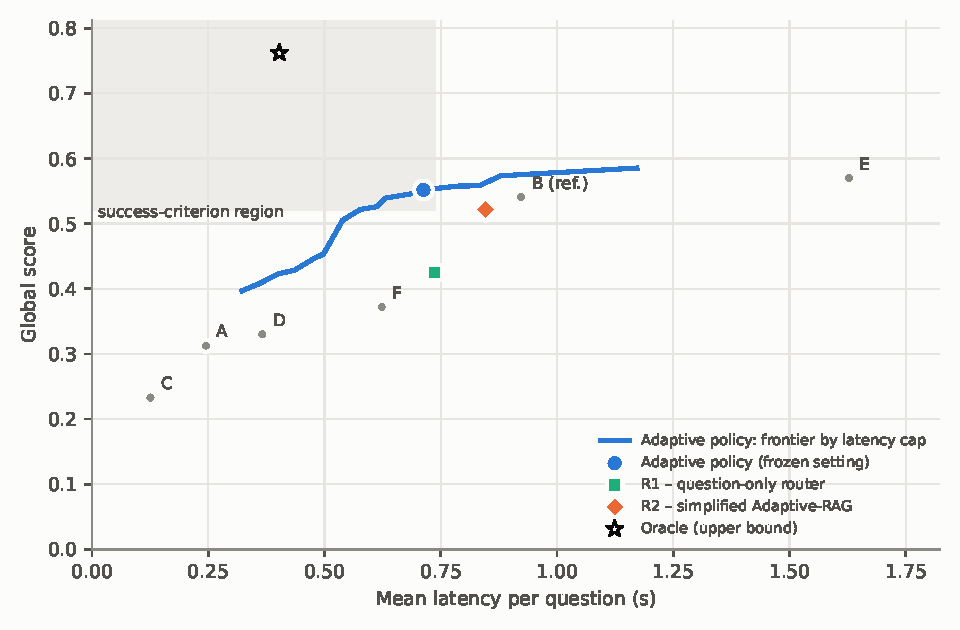
\includegraphics[width=0.78\linewidth]{figures/partie4_qualite_cout_en.pdf}
\caption{Quality--latency trade-off on the development set. The blue curve gives, for each latency cap,
the best score the policy can reach; the blue dot is the frozen setting. The grey area is the success
region.}
\label{fig:dev}
\end{figure}

On the development set, the policy met the primary criterion, with a slight score gain and 23\% less
latency, and it outperformed both routers. Two warning signs were nonetheless visible. Cross-validation
estimated a loss of 2.1 points, right at the limit of the criterion. Above all, simple questions lost
fourteen points in exchange for a twenty-two-point gain on uncovered ones: the robustness criterion was
already not met.

%======================================================================
\section{Final evaluation}\label{sec:final}
%======================================================================

\subsection{Execution conditions}

Once the policy was frozen and published, we ran the six fixed strategies and the policy on the 450 test
questions, in three complete passes. In each pass, the order of methods was randomised to spread the
effect of machine warm-up; the latency kept for each question is the median of the three passes. The
policy was actually executed end to end. Routers R1 and R2, trained on the whole development set, were
applied to the test outputs. Energy was measured throughout the evaluation, more than 30,000 samples in
all, with an idle power of 2.7~W.

Two checks attest to the soundness of the run. Answers are identical from one pass to the next for every
method. And the executed policy reproduces its simulation exactly: the same score on every question, and
the same mean latency to within a thousandth of a second.

\subsection{Results}

\begin{table}[H]
\centering\small\setlength{\tabcolsep}{4pt}
\begin{tabular}{l c c c c c c c}
\toprule
Method & Score & 95\% CI & Gap to B & Latency & P95 & Cov. & Risk \\
\midrule
A -- large, no RAG & 0.310 & [0.269, 0.351] & $-22.7$ & 0.27~s & 0.52~s & 0.45 & 0.76 \\
\textbf{B -- large, 3 passages (ref.)} & \textbf{0.537} & [0.494, 0.581] & -- & \textbf{0.87~s} & 1.26~s & 0.73 & 0.42 \\
C -- small, no RAG & 0.223 & [0.187, 0.261] & $-31.4$ & 0.13~s & 0.25~s & 0.51 & 0.93 \\
D -- small, 3 passages & 0.414 & [0.372, 0.457] & $-12.3$ & 0.35~s & 0.53~s & 0.88 & 0.57 \\
E -- large, 6 passages & 0.567 & [0.523, 0.610] & $+3.0$ & 1.57~s & 2.23~s & 0.75 & 0.40 \\
F -- small, 6 passages & 0.398 & [0.357, 0.440] & $-13.9$ & 0.61~s & 0.87~s & 0.94 & 0.60 \\
\midrule
R1 -- question only & 0.489 & [0.445, 0.534] & $-4.7$ & 0.74~s & 1.61~s & 0.68 & 0.48 \\
R2 -- simplified Adaptive-RAG & 0.517 & [0.473, 0.561] & $-2.0$ & 0.82~s & 1.39~s & 0.68 & 0.44 \\
\textbf{Adaptive policy} & \textbf{0.550} & [0.505, 0.594] & $\mathbf{+1.3}$ & \textbf{0.79~s} & 1.38~s & 0.64 & \textbf{0.40} \\
\midrule
\textit{Oracle} & \textit{0.797} & [0.762, 0.831] & $+26.0$ & \textit{0.36~s} & 1.09~s & 0.64 & 0.18 \\
\bottomrule
\end{tabular}
\caption{Results on the test set (450 questions). Latency is the mean, over questions, of the median of
the three passes.}
\label{tab:resultats}
\end{table}

\begin{figure}[H]
\centering
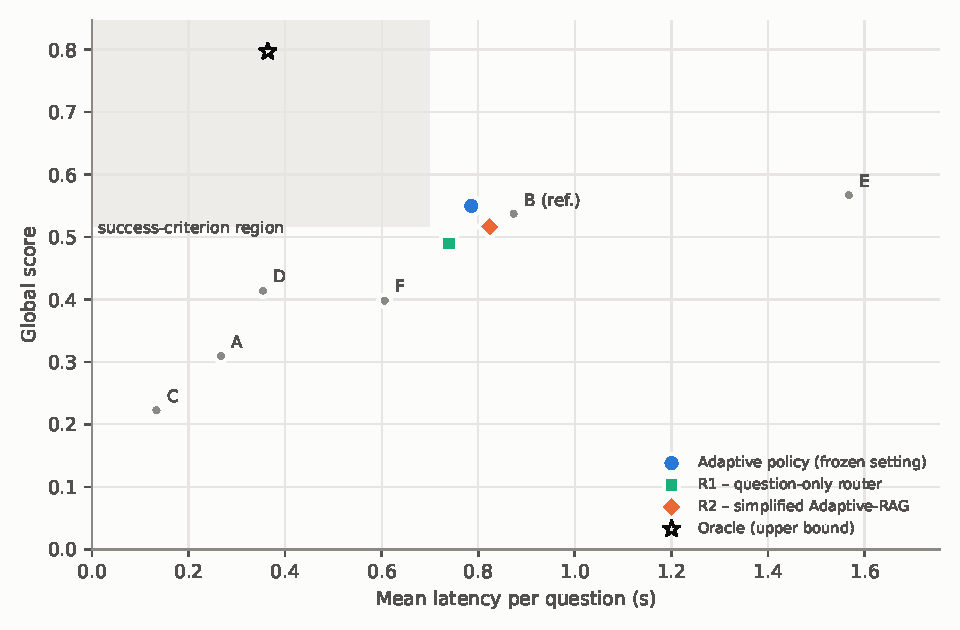
\includegraphics[width=0.78\linewidth]{figures/partie5_qualite_cout_en.pdf}
\caption{Quality--latency trade-off on the test set. The policy (blue) lies above B, but to the right of
the success region.}
\label{fig:test}
\end{figure}

The policy obtains the best score of all feasible methods except E, which is twice as slow. It beats B
by just over one point, makes fewer errors when it answers, and clearly outperforms both routers. But
its mean latency is only 10\% lower than B's.

\subsection{Verdict}

\begin{table}[H]
\centering\small
\begin{tabularx}{\linewidth}{Y >{\centering\arraybackslash}p{5.6cm} c}
\toprule
Criterion & Measurement & Met \\
\midrule
Mean latency reduced by at least 20\% & $-10.1$\% (0.786 vs 0.873~s) & \non \\
Score loss of at most 2~points & gain of 1.3 points & \oui \\
Non-inferiority (upper CI bound of the loss below 2~points) & $[-4.1, +1.6]$ & \oui \\
\textbf{Primary criterion} & & \non \\
\midrule
Risk lower than B & 0.395 vs 0.421 & \oui \\
Better score than R1 and R2 & 0.550 vs 0.489 and 0.517 & \oui \\
No category loses more than 5~points & simple $-7.6$; complex $-3.3$; uncovered $+14.7$ & \non \\
\bottomrule
\end{tabularx}
\caption{Verdict on the pre-registered criteria.}
\label{tab:verdict}
\end{table}

The verdict is therefore mixed. Quality is preserved, non-inferiority is demonstrated, reliability
improves and both reference routers are beaten. But the latency saving reaches only half the target, and
simple questions pay the price of abstention. The main hypothesis, in the form we registered it, is
rejected.

\subsection{Per-category analysis}

\begin{table}[H]
\centering\small
\begin{tabular}{l c c c}
\toprule
Method & Simple & Complex & Uncovered \\
\midrule
B -- reference & 0.737 & 0.468 & 0.407 \\
E -- large, 6 passages & 0.730 & 0.537 & 0.433 \\
R1 & 0.562 & 0.453 & 0.453 \\
R2 & 0.635 & 0.455 & 0.460 \\
\textbf{Adaptive policy} & 0.661 ($-7.6$) & 0.435 ($-3.3$) & \textbf{0.553} ($+14.7$) \\
\textit{Oracle} & 0.842 & 0.682 & 0.867 \\
\bottomrule
\end{tabular}
\caption{Per-category score on the test set (150 questions each). In parentheses, the gap to B in
points.}
\label{tab:categories}
\end{table}

The policy trades quality on answerable questions for reliability on unanswerable ones. Across the 450
questions, it triggered 66 early abstentions and had the large model answer 359 times with three
passages and 25 times with six; 98 of these answers were then replaced by a final abstention. Early
abstentions mostly hit uncovered questions, as intended, but also 18 simple and 12 complex ones: a low
BM25 score does not always mean that the answer is absent.

\subsection{Ablations}

\begin{table}[H]
\centering\small
\begin{tabular}{l c c c c}
\toprule
& \multicolumn{2}{c}{\textbf{Test}} & \multicolumn{2}{c}{\textbf{Development}} \\
\textbf{Variant} (each tuned on development) & Score & Latency & Score & Latency \\
\midrule
\textbf{Full policy} & \textbf{0.550} & 0.79~s & 0.552 & 0.71~s \\
Without adaptive retrieval (always 3 passages) & 0.547 & 0.74~s & 0.548 & 0.68~s \\
Without final abstention & 0.547 & 0.79~s & 0.546 & 0.71~s \\
Without early abstention (small $\to$ large cascade) & 0.464 & 0.64~s & 0.395 & 0.70~s \\
Without any abstention & 0.457 & 0.64~s & 0.389 & 0.70~s \\
\bottomrule
\end{tabular}
\caption{Ablations: each component is removed and the policy is tuned again.}
\label{tab:ablations}
\end{table}

The ablations clearly identify the decisive component: without early abstention, the policy loses almost
nine points on the test set. Adaptive retrieval and final abstention each contribute only three tenths
of a point, within statistical noise. On the test set, always using three passages would even have been
faster, for an equivalent score.

\subsection{Energy}

\begin{table}[H]
\centering\small
\begin{tabular}{l c c c}
\toprule
Method & Energy per question & Gap to B & Mean power \\
\midrule
C -- small, no RAG & 1.8~J & $-90$\% & 16.4~W \\
A -- large, no RAG & 3.9~J & $-80$\% & 17.0~W \\
D -- small, 3 passages & 7.3~J & $-62$\% & 23.2~W \\
F -- small, 6 passages & 13.5~J & $-30$\% & 24.9~W \\
\textbf{Adaptive policy} & \textbf{17.5~J} & $\mathbf{-9}$\% & 24.8~W \\
B -- large, 3 passages (ref.) & 19.3~J & -- & 24.7~W \\
E -- large, 6 passages & 37.7~J & $+95$\% & 26.4~W \\
\bottomrule
\end{tabular}
\caption{Chip energy (CPU, GPU and neural engine) per question on the test set, averaged over the three
passes.}
\label{tab:energie}
\end{table}

Drawn power varies little from one method to another, between 16 and 26~W. Energy therefore essentially
follows computation time, that is, the number of tokens processed, and the policy's saving ($-9$\%)
mirrors its latency reduction. Note in passing that doubling the number of passages almost doubles the
energy, for three points of score.

\subsection{From development to test}

\begin{table}[H]
\centering\small
\begin{tabular}{l c c c c}
\toprule
& \multicolumn{2}{c}{Development (180)} & \multicolumn{2}{c}{Test (450)} \\
Method & Score & Latency & Score & Latency \\
\midrule
B -- reference & 0.541 & 0.92~s & 0.537 & 0.87~s \\
Adaptive policy & 0.552 & 0.71~s ($-23$\%) & 0.550 & 0.79~s ($-10$\%) \\
R1 & 0.425 & 0.74~s & 0.489 & 0.74~s \\
R2 & 0.522 & 0.85~s & 0.517 & 0.82~s \\
Oracle & 0.762 & 0.40~s & 0.797 & 0.36~s \\
\midrule
Early abstentions & \multicolumn{2}{c}{45 / 180 (25\%)} & \multicolumn{2}{c}{66 / 450 (15\%)} \\
\bottomrule
\end{tabular}
\caption{Comparison between the development and test sets.}
\label{tab:dev-test}
\end{table}

Comparing the two sets sheds light on the failure. Quality generalised remarkably well: 0.550 on the test
set, even better than the 0.520 predicted by cross-validation. The latency gain, on the other hand, was
halved. The early-abstention threshold, tuned on sixty questions per category, filtered out a quarter of
the development questions but only 15\% of the test questions. The gap amounts to roughly three standard
errors, which attributes it to the variability of too small a tuning sample. Fewer early abstentions mean
more calls to the large model, and hence a latency closer to that of B.

%======================================================================
\section{Discussion}\label{sec:discussion}
%======================================================================

\subsection{Revisiting the hypotheses}

The first hypothesis is rejected. No signal computed before generation made it possible to send
questions to the small model without loss: R1 loses between five and twelve points depending on the set,
and the tuned policy discarded the small model. The second is not confirmed. The policy makes fewer
errors than B, but model confidence adds almost nothing to the evidence: without final abstention, score
and risk are practically unchanged. The third is partially confirmed. No other method is both more
accurate and faster than the policy, which dominates B; but its cost advantage remains modest. The
fourth, finally, is fully confirmed: seven points lost on simple questions, fifteen gained on uncovered
ones. An average alone would have hidden this trade-off.

\subsection{What we take away}

The first lesson is that, in our setting, \emph{what retrieval has found tells us more than the question
itself}. At comparable latency, the policy beats R1 by six points and R2 by three. This result contrasts
with that of \citet{li2026beyond}, for whom retrieval-derived signals do not reliably improve a
query-based router. The difference may lie in the role we give this signal: we do not use it to choose
between several ways of answering, but to decide not to answer at all.

The second lesson is that \emph{abstention makes adaptation pay off}. Generating nothing when the
evidence is weak saves computation and avoids errors in the same move. It is the only component whose
effect clearly exceeds the noise. The third concerns the small model, which did not find its place: its
confidence signals its errors only moderately, and every escalation costs two generations. The last is
an invitation to go further. The oracle reaches almost 0.80 in 0.36~s: the right choices exist, and the
difficulty lies in predicting them.

\subsection{Practical implications}

For anyone deploying a local assistant, these results suggest a simple, low-risk rule: measure evidence
sufficiency, which costs nothing, and abstain when the documents plainly do not contain the terms of the
question. One thus keeps the quality of the full configuration, reduces wrong answers, and saves a little
time and energy. The threshold must, however, be tuned on a representative sample or, better, expressed
as a proportion of questions; otherwise the time saving becomes unpredictable.

%======================================================================
\section{Weaknesses and avenues for improvement}\label{sec:faiblesses}
%======================================================================

An honest evaluation must say what did not work and why. We present the weaknesses of the study here,
from the most consequential to the most minor, and propose an avenue for improvement for each.
Table~\ref{tab:faiblesses} summarises them.

\subsection{Weaknesses of the method}

\paragraph{Absolute thresholds tuned on a small sample.} This is the direct cause of the failure of the
primary criterion. A threshold set on an absolute value of the evidence, from sixty questions per
category, does not trigger the same proportion of abstentions on another question set, and
cross-validation, carried out on the same small sample, could not reveal it. Several remedies are
possible and can be combined: expressing the threshold as a quantile or a budget (``abstain on the $x$\%
of questions with the weakest evidence''), which guarantees the abstention rate and hence the latency;
calibrating it with a conformal method, which offers risk guarantees without distributional assumptions
\citep{hao2026racer}; tuning on at least five hundred questions; and basing the safety margin on the
variability measured by bootstrap rather than on a value fixed in advance.

\paragraph{Simple questions sacrificed.} Early abstention also discards questions that have an answer,
because a rewording or a synonym is enough to bring the lexical score down. Coverage thus falls from 0.73
to 0.64. A finer sufficiency judge, such as a cross-encoder re-ranker or a small inference model, in the
spirit of Corrective RAG \citep{yan2024crag} and Tiny-Critic RAG \citep{wu2026tinycritic}, should reduce
these false negatives. Combining lexical and dense evidence would help in the same way, as would an
explicit per-category constraint during tuning.

\paragraph{Weak confidence signals.} No signal exceeds an AUC of 0.74, and final abstention contributes
almost nothing. The token probabilities of an answer a few words long say little about its correctness.
Semantic entropy \citep{kuhn2023semantic} or consistency across a few sampled answers would be more
informative; to contain their cost, they could be reserved for borderline cases. A probe trained on the
model's internal states \citep{kadavath2022know} is another avenue.

\paragraph{Adaptive retrieval without effect.} Moving from three to six passages concerns only 6\% of
questions and brings no measurable benefit. Yet complex questions have a recall@3 of only 0.37: the
problem is not the number of passages but retrieval itself. Decomposing multi-step questions, triggering
iterative retrieval when the model hesitates \citep{jiang2023flare,su2024dragin} and compressing the
context to reduce the cost of extra passages \citep{arefeen2024leancontext} would be more promising.

\paragraph{An unused small model.} The final policy uses only one model, so the ``model choice''
dimension of our problem is not really exploited. A stronger small model, or one specialised in
extraction, could change the picture. It could also be given a less demanding role, such as query
reformulation, or used for speculative decoding, where the small model speeds up the large one without
changing its answers.

\paragraph{Degraded tail latency and a persistent gap to the oracle.} The 95th percentile of the
policy's latency (1.38~s) exceeds that of B (1.26~s) because of six-passage answers; it should be included
in the tuning objective. As for the twenty-five-point gap to the oracle, only a learned router combining
question, evidence and confidence, trained on far more data, could hope to narrow it substantially.

\subsection{Weaknesses of the protocol}

\paragraph{A constructed and limited benchmark.} Questions are in English, drawn from two academic
datasets, and query a closed corpus of 3,293 passages. Uncovered questions are adversarial SQuAD 2.0
questions written to resemble the passages, which does not reflect real use. The ambiguous-question
category was not built. Adding MuSiQue \citep{trivedi2022musique} and the CRAG Benchmark
\citep{yang2024cragbench}, a real French-language corpus and some fifty hand-annotated ambiguous questions
would considerably broaden the scope of the conclusions.

\paragraph{A lexical metric.} F1 penalises correct answers phrased differently, whether a paraphrase, a
synonym or a date written another way. A semantic judge, an inference model or an LLM evaluator,
validated on a hand-annotated sample, would give a more faithful picture.

\paragraph{Limited statistical power.} With 450 questions, the confidence interval of the score spans
about four and a half points on either side of the estimate: a two-point difference, the very threshold
of our criterion, cannot be detected with certainty. A test set of at least 1,500 questions would be
needed.

\paragraph{A single device, a single measurement.} All measurements come from the same device, with a
single inference engine and a single quantisation, and energy is that of the chip rather than wall-plug
consumption. Replicating the study on GPUs and with \texttt{llama.cpp}, measuring with a power meter and
reporting memory would consolidate the conclusions on cost.

\paragraph{Design explored on the development set.} Two designs were tried before freezing the policy.
This is documented, but it increases the risk of overfitting the development set. In future, the family
of candidate policies should also be pre-registered, and any improvement should be evaluated on a fresh
test set, this one now being spent.

\paragraph{A review to be deepened.} Our state of the art relies largely on paper abstracts. A full
reading of the closest works (Adaptive-RAG, \citealp{moskvoretskii2025adaptive}, RAGRouter-Bench, RACER
and \citealp{li2026beyond}) is needed to confirm the positioning proposed in
Table~\ref{tab:positionnement}.

\begin{table}[H]
\centering\small
\begin{tabularx}{\linewidth}{Y Y c}
\toprule
Weakness & Main improvement & Priority \\
\midrule
Absolute thresholds, small tuning set & Quantile or budget thresholds, conformal calibration, at least 500 questions & High \\
Loss on simple questions & Lightweight sufficiency judge, per-category constraint & High \\
Limited statistical power & Test set of at least 1,500 questions & High \\
Weak confidence signals & Sampling consistency on borderline cases & Medium \\
Adaptive retrieval without effect & Decomposition of multi-step questions & Medium \\
Limited benchmark & MuSiQue, CRAG, French corpus, ambiguous questions & Medium \\
Lexical metric & Validated semantic judge & Medium \\
Unused small model & Other small model, speculative decoding & Medium \\
Review based on abstracts & Full reading of the closest works & Medium \\
Tail latency & 95th percentile in the tuning objective & Low \\
Gap to the oracle & Learned multi-signal router & Low \\
Single device & Replication on GPU, power meter & Low \\
Exploration on development & Pre-register the policy family & Low \\
\bottomrule
\end{tabularx}
\caption{Summary of weaknesses and proposed improvements.}
\label{tab:faiblesses}
\end{table}

%======================================================================
\section{Conclusion}\label{sec:conclusion}
%======================================================================

We started from a practical question: how can an assistant running on a personal machine spend its
resources wisely, giving each question the effort it deserves? To answer it, we built a benchmark and a
protocol whose success criteria were fixed in advance, established solid references, and then designed
a policy that jointly decides on the model, the number of passages and abstention, based on evidence
sufficiency and model confidence.

The outcome is mixed, and we report it as such. On the test set, the policy preserves the quality of the
reference configuration, makes fewer errors and outperforms two routers inspired by the literature. But
it reduces latency by only 10\% and energy by 9\%, instead of the hoped-for 20\%. We know the cause: an
absolute threshold, tuned on too small a sample, which fired less often on new questions.

Two ideas seem to us to survive this result. On a local machine, the quality of the retrieved evidence
is a safer guide than the wording of the question. And knowing when to abstain is what makes it possible
to save resources without giving up reliability. The next step is to make this lever stable: express
abstention as a calibrated budget, judge evidence sufficiency more finely, and validate the whole on a
larger and entirely fresh test set.

\paragraph{Reproducibility.} The code, the benchmark and the fingerprints of its data, the frozen
configurations (tags \texttt{protocole-v1.0} and \texttt{politique-v1.0}), the raw outputs of the three
passes and the energy measurements are published in the repository given on the first page.

\bibliographystyle{plainnat}
\bibliography{references}

\end{document}
